\documentclass[]{article}
\usepackage{lmodern}
\usepackage{amssymb,amsmath}
\usepackage{ifxetex,ifluatex}
\usepackage{fixltx2e} % provides \textsubscript
\ifnum 0\ifxetex 1\fi\ifluatex 1\fi=0 % if pdftex
  \usepackage[T1]{fontenc}
  \usepackage[utf8]{inputenc}
\else % if luatex or xelatex
  \ifxetex
    \usepackage{mathspec}
  \else
    \usepackage{fontspec}
  \fi
  \defaultfontfeatures{Ligatures=TeX,Scale=MatchLowercase}
\fi
% use upquote if available, for straight quotes in verbatim environments
\IfFileExists{upquote.sty}{\usepackage{upquote}}{}
% use microtype if available
\IfFileExists{microtype.sty}{%
\usepackage{microtype}
\UseMicrotypeSet[protrusion]{basicmath} % disable protrusion for tt fonts
}{}
\usepackage[margin=1in]{geometry}
\usepackage{hyperref}
\hypersetup{unicode=true,
            pdftitle={Assessment 03 - Distribution},
            pdfauthor={Gabriele Mineo - Harvard Data Science Professional},
            pdfborder={0 0 0},
            breaklinks=true}
\urlstyle{same}  % don't use monospace font for urls
\usepackage{graphicx,grffile}
\makeatletter
\def\maxwidth{\ifdim\Gin@nat@width>\linewidth\linewidth\else\Gin@nat@width\fi}
\def\maxheight{\ifdim\Gin@nat@height>\textheight\textheight\else\Gin@nat@height\fi}
\makeatother
% Scale images if necessary, so that they will not overflow the page
% margins by default, and it is still possible to overwrite the defaults
% using explicit options in \includegraphics[width, height, ...]{}
\setkeys{Gin}{width=\maxwidth,height=\maxheight,keepaspectratio}
\IfFileExists{parskip.sty}{%
\usepackage{parskip}
}{% else
\setlength{\parindent}{0pt}
\setlength{\parskip}{6pt plus 2pt minus 1pt}
}
\setlength{\emergencystretch}{3em}  % prevent overfull lines
\providecommand{\tightlist}{%
  \setlength{\itemsep}{0pt}\setlength{\parskip}{0pt}}
\setcounter{secnumdepth}{0}
% Redefines (sub)paragraphs to behave more like sections
\ifx\paragraph\undefined\else
\let\oldparagraph\paragraph
\renewcommand{\paragraph}[1]{\oldparagraph{#1}\mbox{}}
\fi
\ifx\subparagraph\undefined\else
\let\oldsubparagraph\subparagraph
\renewcommand{\subparagraph}[1]{\oldsubparagraph{#1}\mbox{}}
\fi

%%% Use protect on footnotes to avoid problems with footnotes in titles
\let\rmarkdownfootnote\footnote%
\def\footnote{\protect\rmarkdownfootnote}

%%% Change title format to be more compact
\usepackage{titling}

% Create subtitle command for use in maketitle
\newcommand{\subtitle}[1]{
  \posttitle{
    \begin{center}\large#1\end{center}
    }
}

\setlength{\droptitle}{-2em}

  \title{Assessment 03 - Distribution}
    \pretitle{\vspace{\droptitle}\centering\huge}
  \posttitle{\par}
    \author{Gabriele Mineo - Harvard Data Science Professional}
    \preauthor{\centering\large\emph}
  \postauthor{\par}
    \date{}
    \predate{}\postdate{}
  

\begin{document}
\maketitle

\subsection{\texorpdfstring{\textbf{Distributions -
1}}{Distributions - 1}}\label{distributions---1}

You may have noticed that numerical data is often summarized with the
average value. For example, the quality of a high school is sometimes
summarized with one number: the average score on a standardized test.
Occasionally, a second number is reported: the standard deviation. So,
for example, you might read a report stating that scores were 680 plus
or minus 50 (the standard deviation). The report has summarized an
entire vector of scores with with just two numbers. Is this appropriate?
Is there any important piece of information that we are missing by only
looking at this summary rather than the entire list? We are going to
learn when these 2 numbers are enough and when we need more elaborate
summaries and plots to describe the data.

Our first data visualization building block is learning to summarize
lists of factors or numeric vectors. The most basic statistical summary
of a list of objects or numbers is its distribution. Once a vector has
been summarized as distribution, there are several data visualization
techniques to effectively relay this information. In later assessments
we will practice to write code for data visualization. Here we start
with some multiple choice questions to test your understanding of
distributions and related basic plots.

In the murders dataset, the region is a categorical variable and on the
right you can see its distribution. To the closet 5\%, what proportion
of the states are in the North Central region?

\begin{figure}
\centering
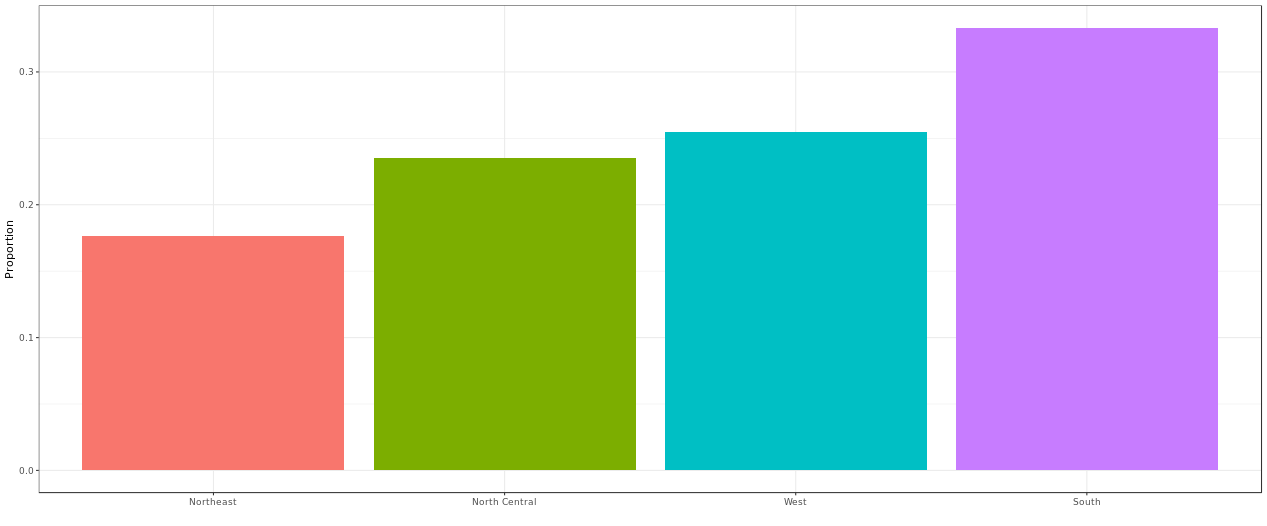
\includegraphics{img1.png}
\caption{}
\end{figure}

Possible Answers

\begin{itemize}
\tightlist
\item
  75\%
\item
  50\%
\item
  20\% {[}X{]}
\item
  5\%
\end{itemize}

\subsection{\texorpdfstring{\textbf{Distributions -
2}}{Distributions - 2}}\label{distributions---2}

In the murders dataset, the region is a categorical variable and to the
right is its distribution.

Which of the following is true:

\begin{figure}
\centering
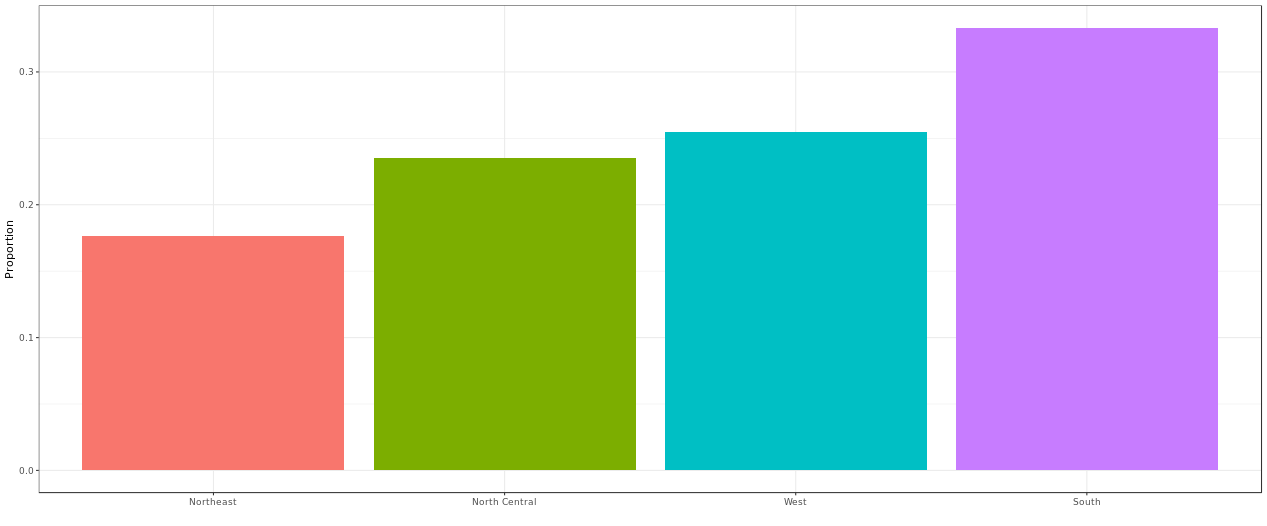
\includegraphics{img1.png}
\caption{}
\end{figure}

Possible Answers

\begin{itemize}
\tightlist
\item
  The graph is a histogram.
\item
  The graph shows only four numbers with a bar plot. {[}X{]}
\item
  Categories are not numbers so it does not make sense to graph the
  distribution.
\item
  The colors, not the height of the bars, describe the distribution.
\end{itemize}

\subsection{\texorpdfstring{\textbf{Empirical Cumulative Distribution
Function
(eCDF)}}{Empirical Cumulative Distribution Function (eCDF)}}\label{empirical-cumulative-distribution-function-ecdf}

The plot shows the eCDF for male heights:

\begin{figure}
\centering
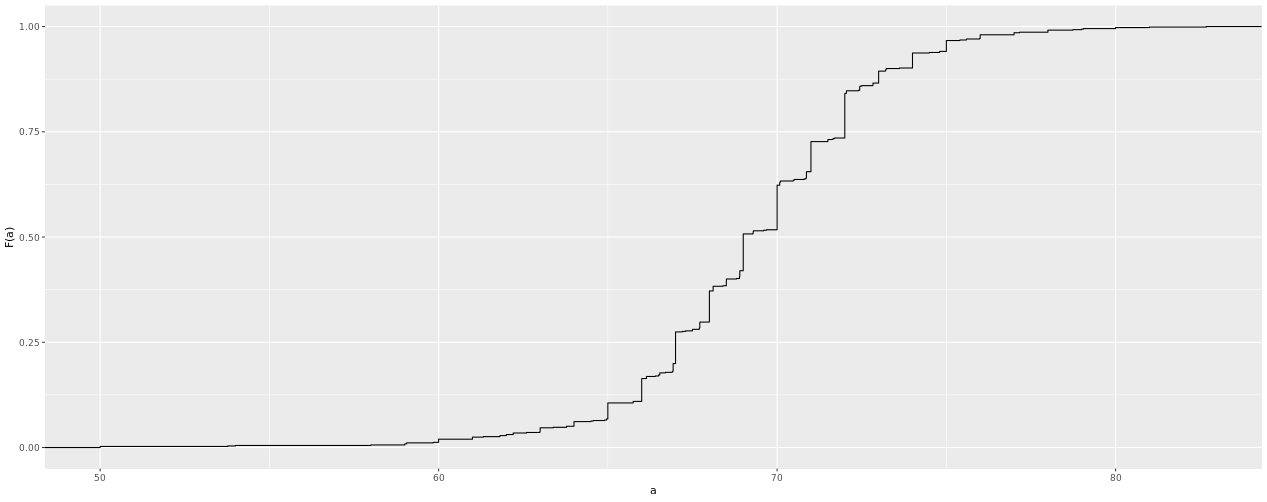
\includegraphics{img2.png}
\caption{}
\end{figure}

Based on the plot, what percentage of males are shorter than 75 inches?

Possible Answers

\begin{itemize}
\tightlist
\item
  100\%
\item
  95\% {[}X{]}
\item
  80\%
\item
  72 inches
\end{itemize}

\subsection{\texorpdfstring{\textbf{eCDF Male
Heights}}{eCDF Male Heights}}\label{ecdf-male-heights}

The plot shows the eCDF for male heights:

\begin{figure}
\centering
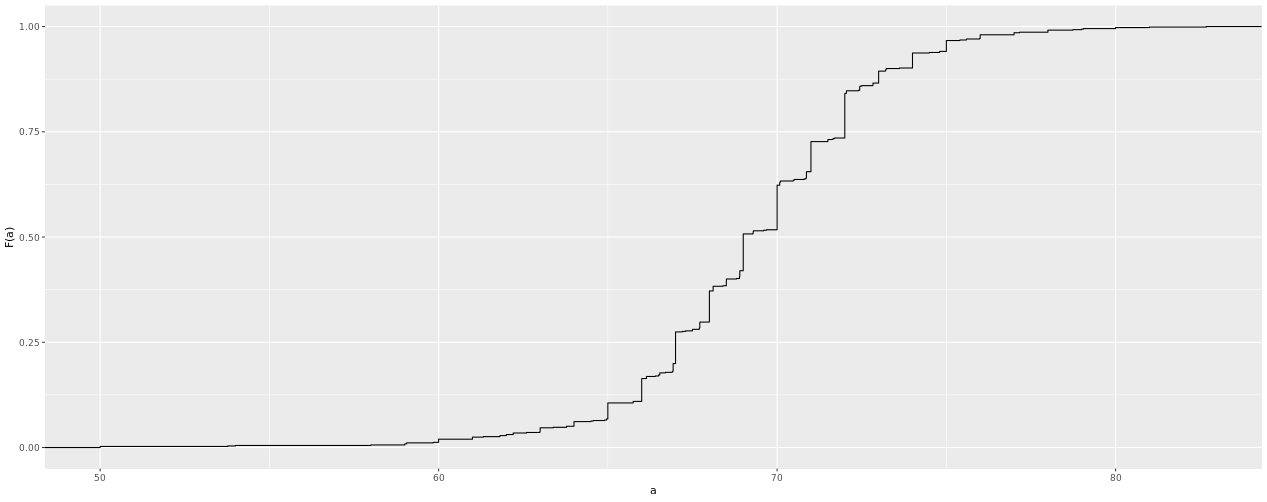
\includegraphics{img2.png}
\caption{}
\end{figure}

To the closest inch, what height m has the property that 1/2 of the male
students are taller than m and 1/2 are shorter?

Possible Answers

\begin{itemize}
\tightlist
\item
  61 inches
\item
  64 inches
\item
  69 inches {[}X{]}
\item
  74 inches
\end{itemize}

\subsection{\texorpdfstring{\textbf{eCDF of Murder
Rates}}{eCDF of Murder Rates}}\label{ecdf-of-murder-rates}

Here is an eCDF of the murder rates across states.

\begin{figure}
\centering
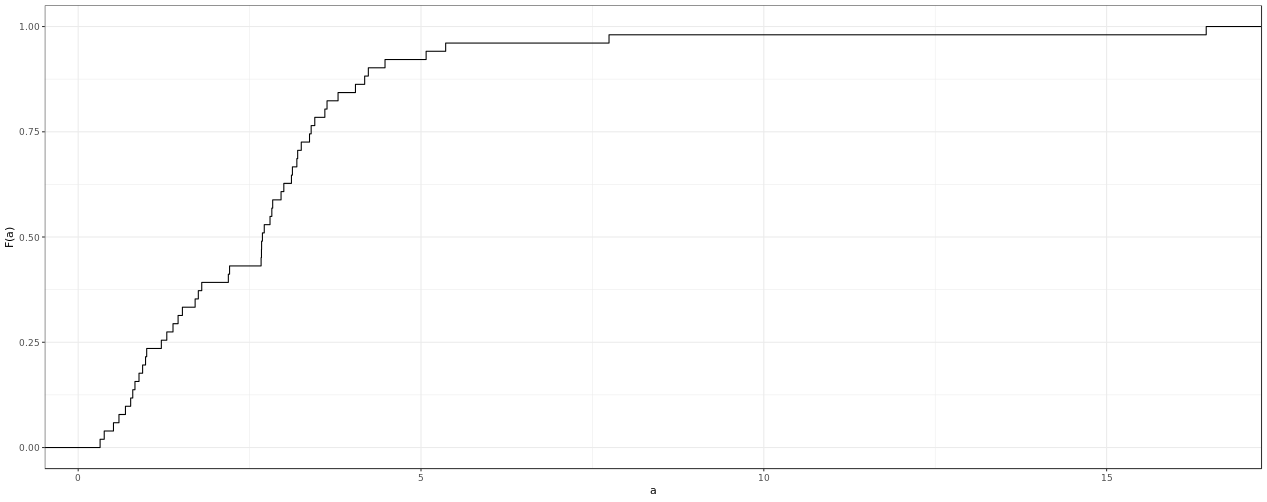
\includegraphics{img3.png}
\caption{}
\end{figure}

Knowing that there are 51 states (counting DC) and based on this plot,
how many states have murder rates larger than 10 per 100,000 people?

Possible Answers

\begin{itemize}
\tightlist
\item
  1 {[}X{]}
\item
  5
\item
  10
\item
  50
\end{itemize}

\subsection{\texorpdfstring{\textbf{eCDF of Murder Rates -
2}}{eCDF of Murder Rates - 2}}\label{ecdf-of-murder-rates---2}

Here is an eCDF of the murder rates across states:

\begin{figure}
\centering
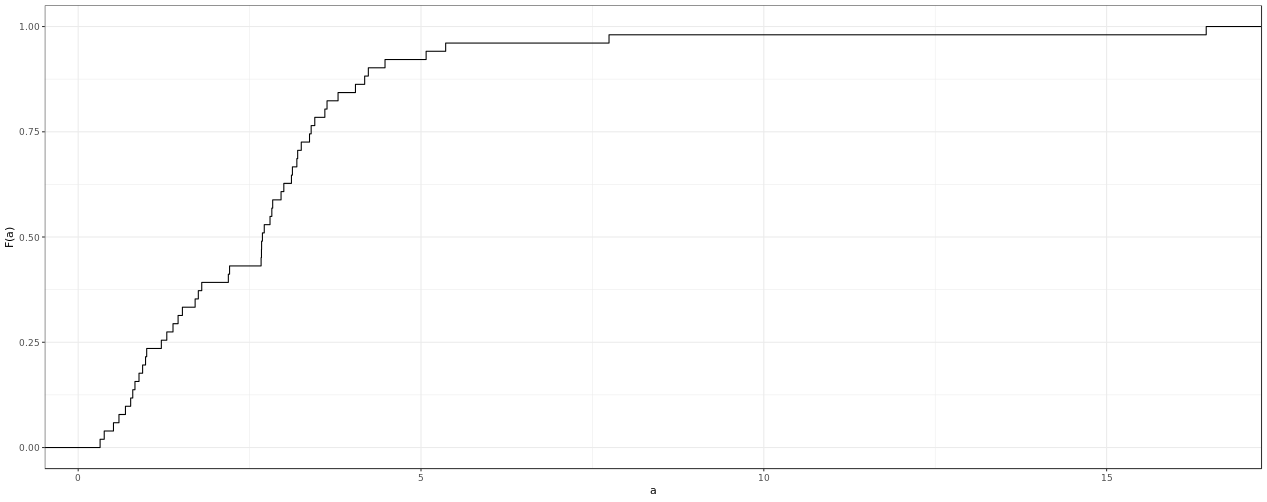
\includegraphics{img3.png}
\caption{}
\end{figure}

Based on the eCDF above, which of the following statements are true:

Possible Answers

\begin{itemize}
\tightlist
\item
  About half the states have murder rates above 7 per 100,000 and the
  other half below.
\item
  Most states have murder rates below 2 per 100,000.
\item
  All the states have murder rates above 2 per 100,000.
\item
  With the exception of 4 states, the murder rates are below 5 per
  100,000. {[}X{]}
\end{itemize}

\subsection{\texorpdfstring{\textbf{Histograms}}{Histograms}}\label{histograms}

Here is a histogram of male heights in our heights dataset:

\begin{figure}
\centering
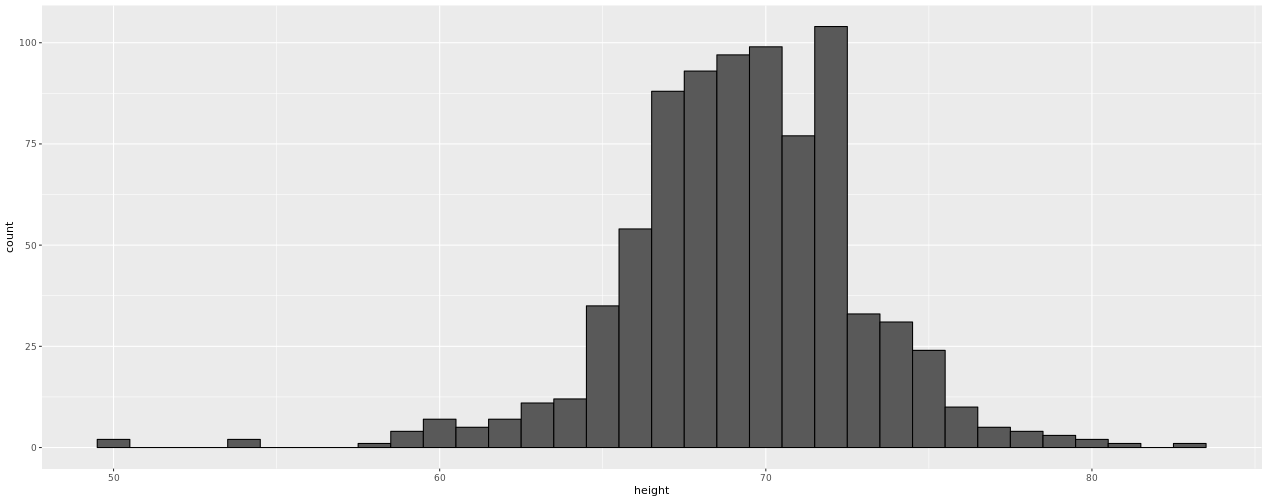
\includegraphics{img4.png}
\caption{}
\end{figure}

Based on this plot, how many males are between 62.5 and 65.5?

Possible Answers

\begin{itemize}
\tightlist
\item
  5
\item
  24
\item
  44 {[}X{]}
\item
  100
\end{itemize}

\subsection{\texorpdfstring{\textbf{Histograms -
2}}{Histograms - 2}}\label{histograms---2}

Here is a histogram of male heights in our heights dataset:

\begin{figure}
\centering
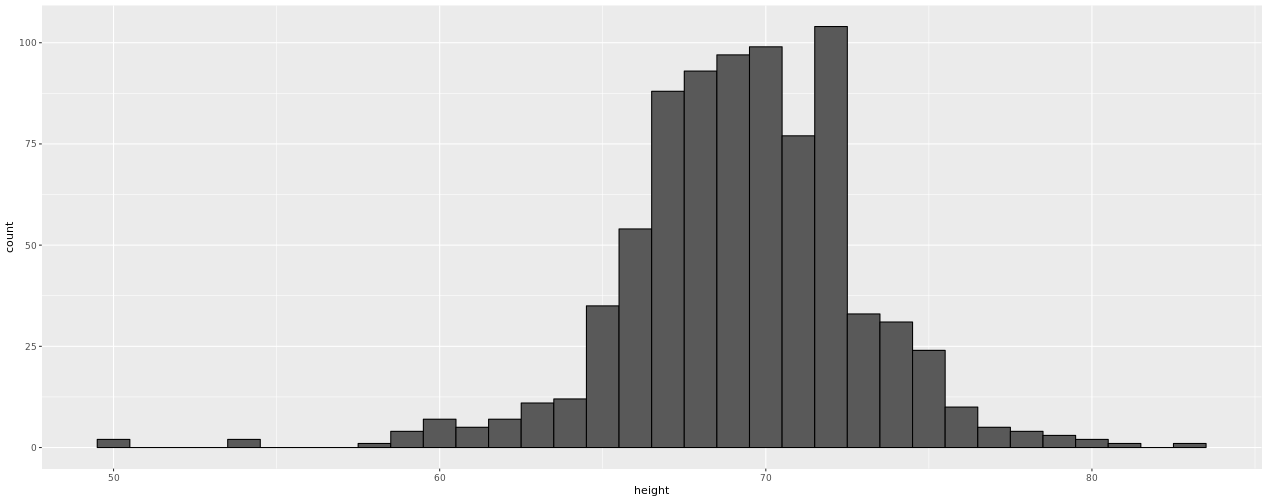
\includegraphics{img4.png}
\caption{}
\end{figure}

About what percentage are shorter than 60 inches?

Possible Answers

\begin{itemize}
\tightlist
\item
  1\% {[}X{]}
\item
  10\%
\item
  25\%
\item
  50\%
\end{itemize}

\subsection{\texorpdfstring{\textbf{Density
plots}}{Density plots}}\label{density-plots}

Based on this density plot, about what proportion of US states have
populations larger than 10 million?

\begin{figure}
\centering
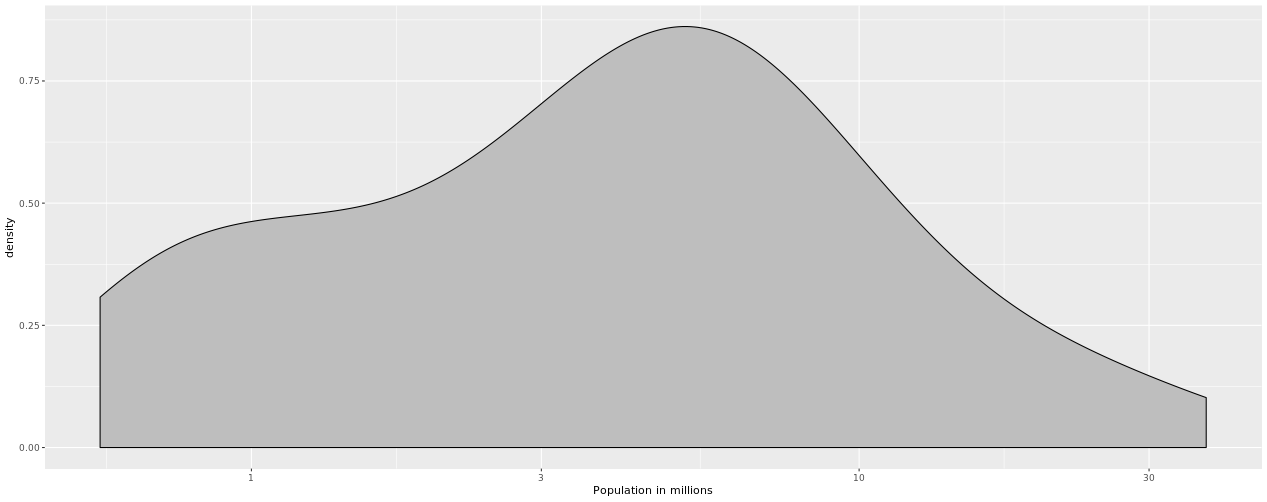
\includegraphics{img5.png}
\caption{}
\end{figure}

Possible Answers

\begin{itemize}
\tightlist
\item
  0.02
\item
  0.15 {[}X{]}
\item
  0.50
\item
  0.55
\end{itemize}

\subsection{\texorpdfstring{\textbf{Density plots -
2}}{Density plots - 2}}\label{density-plots---2}

Here are three density plots. Is it possible that they are from the same
dataset? Which of the following statements is true:

\begin{figure}
\centering
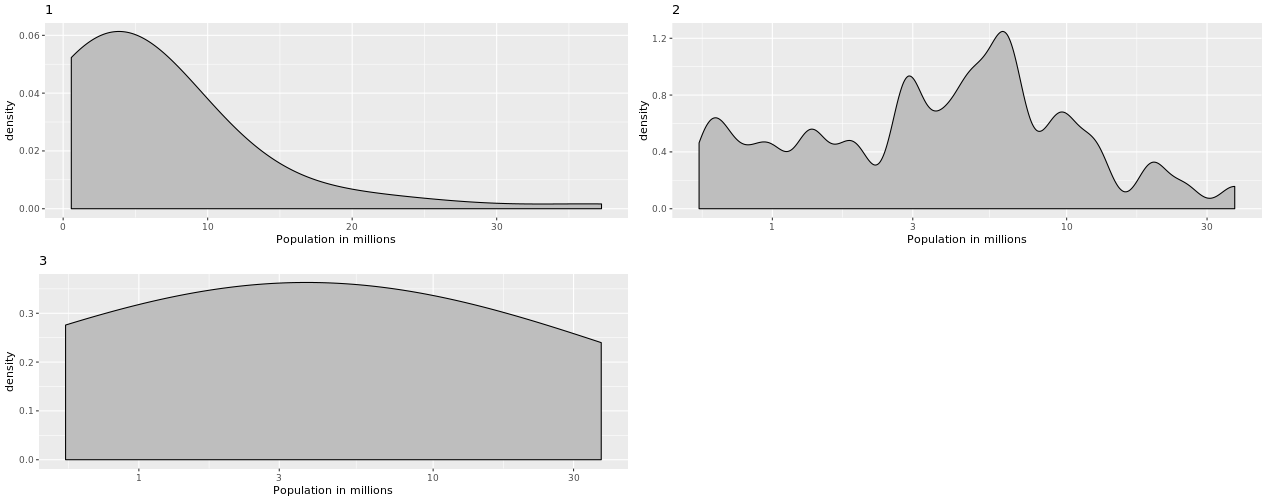
\includegraphics{img6.png}
\caption{}
\end{figure}

Possible Answers

\begin{itemize}
\tightlist
\item
  It is impossible that they are from the same dataset.
\item
  They are from the same dataset, but different due to code errors.
\item
  They are the same dataset, but the first and second undersmooth and
  the third oversmooths.
\item
  They are the same dataset, but the first is not in the log scale, the
  second undersmooths and the third oversmooths. {[}X{]}
\end{itemize}


\end{document}
